


\tikzset{every picture/.style={line width=0.75pt}} %set default line width to 0.75pt        

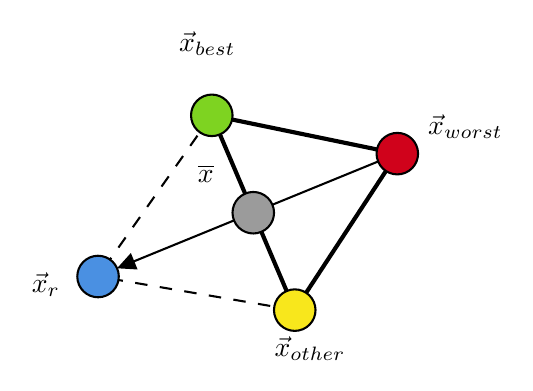
\begin{tikzpicture}[x=0.75pt,y=0.75pt,yscale=-1,xscale=1]
%uncomment if require: \path (0,914); %set diagram left start at 0, and has height of 914

%Straight Lines [id:da39121424549824235] 
\draw [line width=1.5]    (122.21,293.73) -- (211.59,312.19) ;
%Straight Lines [id:da618739710662245] 
\draw [line width=1.5]    (162.18,387.58) -- (122.21,293.73) ;
%Straight Lines [id:da7599011924098371] 
\draw [line width=1.5]    (162.18,387.58) -- (211.59,312.19) ;
%Straight Lines [id:da920148193557524] 
\draw    (211.59,312.19) -- (79.35,366.27) ;
\draw [shift={(76.58,367.41)}, rotate = 337.75] [fill={rgb, 255:red, 0; green, 0; blue, 0 }  ][line width=0.08]  [draw opacity=0] (8.93,-4.29) -- (0,0) -- (8.93,4.29) -- cycle    ;
%Shape: Circle [id:dp8356416145204131] 
\draw  [fill={rgb, 255:red, 155; green, 155; blue, 155 }  ,fill opacity=1 ] (132.99,344.57) .. controls (130.83,339.49) and (133.2,333.62) .. (138.28,331.45) .. controls (143.36,329.29) and (149.23,331.65) .. (151.4,336.74) .. controls (153.56,341.82) and (151.19,347.69) .. (146.11,349.85) .. controls (141.03,352.02) and (135.16,349.65) .. (132.99,344.57) -- cycle ;
%Shape: Circle [id:dp45226827899303657] 
\draw  [fill={rgb, 255:red, 208; green, 2; blue, 27 }  ,fill opacity=1 ] (202.39,316.1) .. controls (200.22,311.02) and (202.59,305.15) .. (207.67,302.99) .. controls (212.75,300.82) and (218.62,303.19) .. (220.79,308.27) .. controls (222.95,313.35) and (220.59,319.22) .. (215.51,321.39) .. controls (210.43,323.55) and (204.55,321.19) .. (202.39,316.1) -- cycle ;
%Straight Lines [id:da7153645519608796] 
\draw  [dash pattern={on 4.5pt off 4.5pt}]  (162.18,387.58) -- (67.4,371.39) ;
%Straight Lines [id:da799114901839753] 
\draw  [dash pattern={on 4.5pt off 4.5pt}]  (122.21,293.73) -- (67.4,371.39) ;
%Shape: Circle [id:dp5444502759814949] 
\draw  [fill={rgb, 255:red, 74; green, 144; blue, 226 }  ,fill opacity=1 ] (76.58,367.41) .. controls (78.77,372.47) and (76.45,378.36) .. (71.38,380.56) .. controls (66.32,382.76) and (60.43,380.43) .. (58.23,375.37) .. controls (56.03,370.3) and (58.36,364.41) .. (63.42,362.21) .. controls (68.49,360.01) and (74.38,362.34) .. (76.58,367.41) -- cycle ;
%Shape: Circle [id:dp26683593943410067] 
\draw  [fill={rgb, 255:red, 126; green, 211; blue, 33 }  ,fill opacity=1 ] (113.01,297.65) .. controls (110.85,292.57) and (113.21,286.7) .. (118.29,284.53) .. controls (123.37,282.37) and (129.25,284.73) .. (131.41,289.81) .. controls (133.57,294.9) and (131.21,300.77) .. (126.13,302.93) .. controls (121.05,305.1) and (115.17,302.73) .. (113.01,297.65) -- cycle ;
%Shape: Circle [id:dp8150487348338344] 
\draw  [fill={rgb, 255:red, 248; green, 231; blue, 28 }  ,fill opacity=1 ] (152.98,391.49) .. controls (150.82,386.41) and (153.18,380.54) .. (158.26,378.38) .. controls (163.34,376.21) and (169.22,378.58) .. (171.38,383.66) .. controls (173.54,388.74) and (171.18,394.61) .. (166.1,396.78) .. controls (161.02,398.94) and (155.14,396.58) .. (152.98,391.49) -- cycle ;

% Text Node
\draw (105,252) node [anchor=north west][inner sep=0.75pt]   [align=left] {$\displaystyle \vec{x}_{best}$};
% Text Node
\draw (225,292) node [anchor=north west][inner sep=0.75pt]   [align=left] {$\displaystyle \vec{x}_{worst}$};
% Text Node
\draw (151,399) node [anchor=north west][inner sep=0.75pt]   [align=left] {$\displaystyle \vec{x}_{other}$};
% Text Node
\draw (114,316) node [anchor=north west][inner sep=0.75pt]   [align=left] {$\displaystyle \overline{x}$};
% Text Node
\draw (34,368) node [anchor=north west][inner sep=0.75pt]   [align=left] {$\displaystyle \vec{x}_{r}$};


\end{tikzpicture}